% Generated by scripts/2026-10-21/extract_floats.py from paper/main_en.tex; edit the full manuscript, not this file.
\begin{figure}[htbp]
\centering
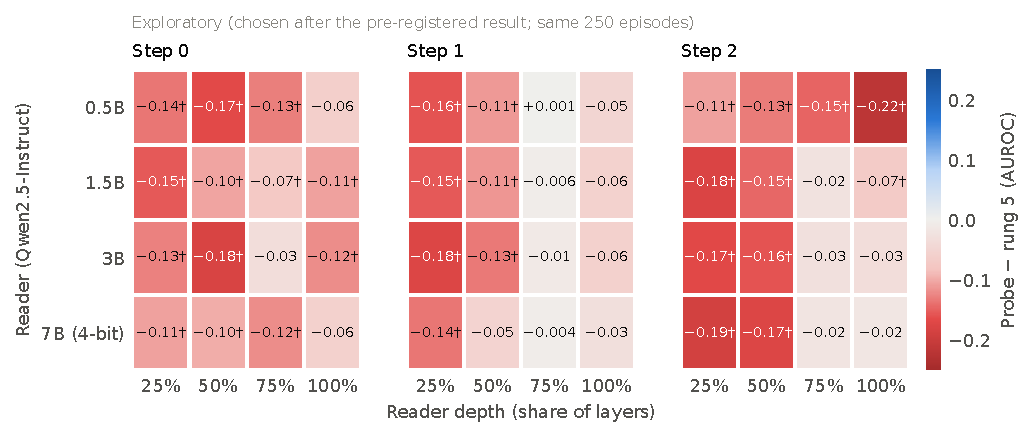
\includegraphics[width=\linewidth]{fig4_reader_depth.pdf}
\caption{Exploratory: probe $-$ rung 5 AUROC difference for every reader $\times$ depth of the linear probe on the first 250 episodes (48 cells, no selection). Diverging color centered on zero (red: probe below rung 5); $\dagger$ marks cells whose 95\% CI (scene-level cluster bootstrap) excludes zero, all of them below zero (31 of 48). No cell's CI lies above zero; the largest difference is $+0.001$. The 7B reader used 4-bit weights, so size is confounded with quantization. Linear and MLP cells with CIs: Appendix Table~\ref{tab:a9}.}\label{fig:heat}
% Source: results/explore_{0.5B,1.5B,3B,7B-4bit}_diff.csv
\end{figure}
